\documentclass[]{article}
\usepackage{amsmath}
\usepackage{graphicx}
%opening
\title{Problem Set 2}
\author{Zixuan Huang}

\begin{document}

\maketitle
Code is also posted on my GitHub page: https://github.com/zhuang13atJHU/Numeric-Analysis/tree/master  
\section{discretizing the AR(1) income process}
Using equations in the lecture notes, we can construct the transition matrix with five states of income. See code for details. 
\section{cake-eating problem with uncertain income}
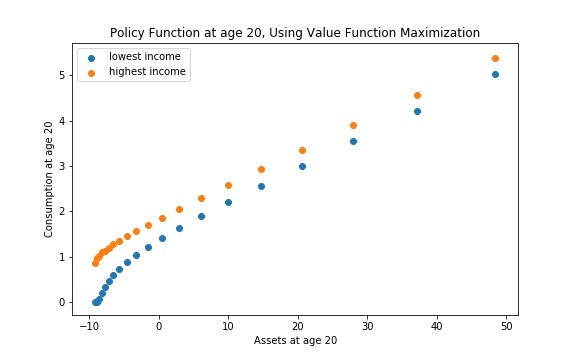
\includegraphics[width=\linewidth]{value func.jpg}
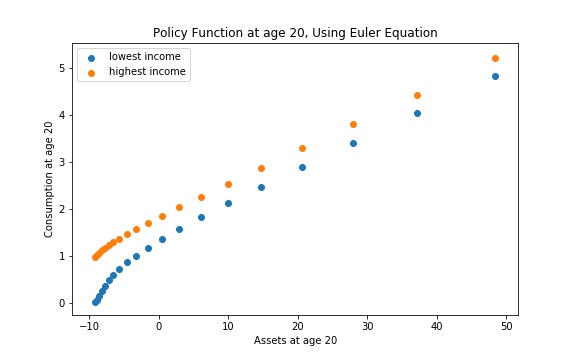
\includegraphics[width=\linewidth]{Euler no trans.jpg}
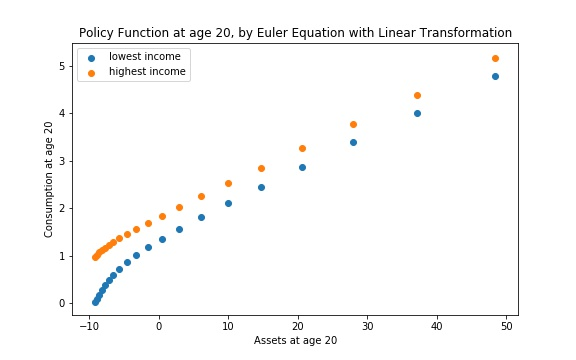
\includegraphics[width=\linewidth]{Euler.jpg}
\section{computing simulated moments on consumption and asset}
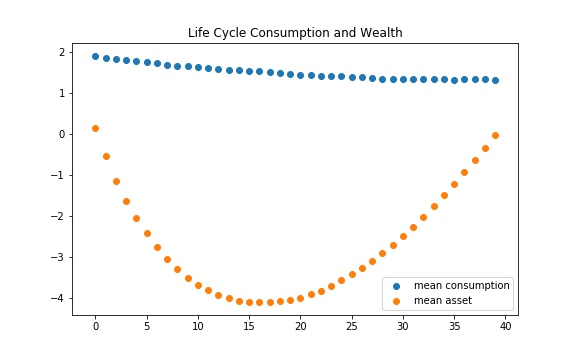
\includegraphics[width=\linewidth]{LifeCycle.jpg}
Comments on Q2 and Q3:
\begin{itemize}
	\item Over time
	\begin{itemize}
		\item Consumption smoothness: since households are allowed to borrow, they would like to smooth consumption due to impatience
		\item Saving: in order to smooth consumption, households borrow at the early stage of their life, and accumulate wealth when they are getting old. 
		\item Concavity of consumption function: due to precautionary motive, marginal propensity to consume is larger when they are poor than when they are rich. This provides policy implications for government when redistributing wealth across different groups of people. 
	\end{itemize}
	\item Across income shocks
	\begin{itemize}
		\item Level of income: people with the same wealth level behave differently when receiving different incomes. 
		\item Expectation: the fact that people who earns more consume more is not just because they receive more, but also because they expect to earn more in the future due to the AR process. That is, in the world of uncertainty, expectation does play a significant role in influencing behaviors and decision making.
	\end{itemize}
	\item Representative and heterogenous agent
	\begin{itemize}
		\item Heterogeneity: the model is heterogenous in the sense that households receive idiosyncratic income shocks and thus have different wealth level.
		\item  Representativity: however, all individuals have the same homothetic preference(homogenous utility function, and they share the same beta), so the economy as a whole behaves like a representative agent.
	\end{itemize}
\end{itemize}

\end{document}
